
%%%%%%%%%%%%%%%%%%%%%%% file typeinst.tex %%%%%%%%%%%%%%%%%%%%%%%%%
%
% This is the LaTeX source for the instructions to authors using
% the LaTeX document class 'llncs.cls' for contributions to
% the Lecture Notes in Computer Sciences series.
% http://www.springer.com/lncs       Springer Heidelberg 2006/05/04
%
% It may be used as a template for your own input - copy it
% to a new file with a new name and use it as the basis
% for your article.
%
% NB: the document class 'llncs' has its own and detailed documentation, see
% ftp://ftp.springer.de/data/pubftp/pub/tex/latex/llncs/latex2e/llncsdoc.pdf
%
%%%%%%%%%%%%%%%%%%%%%%%%%%%%%%%%%%%%%%%%%%%%%%%%%%%%%%%%%%%%%%%%%%%


\documentclass[runningheads,a4paper]{llncs}

\setcounter{tocdepth}{3}
\usepackage{graphicx}
\usepackage{booktabs}
\usepackage{times}
\usepackage{epsfig}
\usepackage{amsmath}
\usepackage{amssymb}
\usepackage{multirow}
\usepackage{nicefrac}

\usepackage{url}
\urldef{\mailsa}\path|michael.berks@manchester.ac.uk|

\newcommand{\keywords}[1]{\par\addvspace\baselineskip
\noindent\keywordname\enspace\ignorespaces#1}

% macros for referencing figures, tables, equations and sections
\def\figpath{./figs}
\newcommand{\fref}[1]{Figure~\ref{#1}}
\newcommand{\eref}[1]{(\ref{#1})}
\newcommand{\tref}[1]{Table~\ref{#1}}
\newcommand{\sref}[1]{Section~\ref{#1}}
\newcommand{\aref}[1]{Algorithm~\ref{#1}}

% alternatives if booktabs not available
%\newcommand{\toprule}{\hline\noalign{\smallskip}}
%\newcommand{\midrule}[1]{\cline{#1}\noalign{\smallskip}}
%\newcommand{\bottomrule}{\hline\noalign{\smallskip}}

% maths macros
\def\G{G}
\def\Gx{G_x}
\def\Gy{G_y}
\def\Gxx{G_{xx}}
\def\Gxxs{G_{xx}(\sigma)}
\def\Gxy{G_{xy}}
\def\Gxys{G_{xy}(\sigma)}
\def\Gyx{G_{yx}}
\def\Gyy{G_{yy}}
\def\Gyys{G_{yy}(\sigma)}
\def\Ix{I_x}
\def\Iy{I_y}
\def\Ixsqr{I_{x^2}}
\def\Iysqr{I_{y^2}}
\def\Ixx{I_{G_{xx}}}
\def\Ixxs{I_{G_{xx}}(\sigma)}
\def\Ixy{I_{G_{xy}}}
\def\Ixys{I_{G_{xy}}(\sigma)}
\def\Iyy{I_{G_{yy}}}
\def\Iyys{I_{G_{yy}}(\sigma)}
\def\Igt{I_{G_{theta}}}
\def\Iht{I_{H_{theta}}}
\def\dtcwt{DT-$\mathbb{C}$WT}
\def\figpath{./figs}
\def\ie{i.e.}
\def\eg{e.g.}
\def\etc{etc.}
\def\etal{\emph{et al.}}

% command for adding inline comment to text
\newcommand{\comment}[1]{\textbf{[#1]}}
%\newcommand{\comment}[1]{}

\begin{document}

\mainmatter  % start of an individual contribution

% first the title is needed
\title{An Automated System for Detecting and Measuring Nailfold Capillaries}

% a short form should be given in case it is too long for the running head
\titlerunning{Detecting and Measuring Nailfold Capillaries}

% the name(s) of the author(s) follow(s) next
%
% NB: Chinese authors should write their first names(s) in front of
% their surnames. This ensures that the names appear correctly in
% the running heads and the author index.
%
\author{*}%

\institute{*}
\authorrunning{*} % abbreviated author list (for running head)

\toctitle{Lecture Notes in Computer Science}
\tocauthor{}
\maketitle


\begin{abstract}
Abstract here.
\end{abstract}

\section{Introduction}
\label{s:introduction}
Nailfold capillaroscopy is an optical microscopy technique for imaging capillaries in the skin above the fingernail. It can be used to non-invasively detect microvascular abnormalities, and is commonly used in the diagnosis and assessment of systemic sclerosis (SSc), a connective tissue disorder that is painful, disabling and disfiguring, with high mortality. In particular, NC can identify structural changes in capillaries to help differentiate patients with symptoms of Raynaud’s Phenomenon (the most common presenting feature of SSc) from people with the more common and relatively benign primary (idiopathic) RP (PRP).

Typically such structural changes were labelled either as binary outcomes (\eg~normal vs abnormal) or into coarse disease stages (early, active, late), however with the development of drugs with vascular remodelling potential, and increasing interest in (clinical trials of) early intervention, there has been a move towards quantitative assessment of capillary morphology~\cite{Murray_etal_AR09,Paradowski_etal_KES09b,Berks_MICCAI14}. Manual measurements of vessel size, shape and density in NC images have been shown to be more reproducible than qualitative assessment~\cite{Murray_etal_AR09}, show good discrimination between SSc and PRP, and allow the monitoring of disease progression, while recent work has shown such measurements can be made automatically to the same level of accuracy as expert observers~\cite{Berks_MICCAI14}.

However, these \textit{structural} changes happen on a timescale of months/years and may not be useful for monitoring rapid changes, e.g. in a clinical trial of vasoactive therapy. In contrast, imaging of capillary \textit{function} may provide insights into pathophysiology, and markers of disease activity (i.e outcome measures in clinical trials), not only in SSc but in other conditions in which the microvasculature plays a key role including diabetes, tumours (including in animal models), and certain skin lesions (e.g. psoriasis and port wine stains).

We have developed a state-of-the-art NC system that uses a high-frame camera (120 fps) to capture video sequences in which it is possible to measure blood flow velocity in individual capillaries. The system has been designed to allow the fast and easy acquisition of high-magnification (1${\mu}m$ per pixel) video across the whole nailfold, and includes software that generates high-quality static image mosaics (for clinical assessment) and makes fully-automated measures of capillary structure and flow - the latter using a novel optmisied optical flow algorithm developed to be robust to the extremely challenging low-contrast, high-noise conditions inherent in NC imaging. While flow has been estimated previously in NC video [find citation], this was performed only at manually labelled points, an approach that both introduces subjectivity and does not scale to analysing large datasets. We believe our system is the first to measure flow fully-automatically in \textit{all} visible capillaries.

In this paper we describe the new system, and present results of an initial trial in which it was used to image 50 healthy controls, 12 people with PRP and 50 patients with SSc. We show that automated measures of capillary structure can differentiate between patients with SSc and healthy controls/PRP providing further evidence to the validity of the technique, and moreover show that at a combined model provides greater predictive power than individual measures alone. Finally we show that our novel optical flow algorithm measures capillary blood velocity reliably (?) and provides additional independent information to capillary structure.


Some other citations in case we need them (delete later if necessary) ~\cite{Mayes_etal_AR03}, ~\cite{HerrickCOinR2011,HerrickAR2009}, ~\cite{Cutolo_etal_BPRCR08}.

%\newpage
\begin{figure}[t]
\centering
\begin{tabular}{@{}c@{}}
\includegraphics[width=0.98\columnwidth]{\figpath/sequence_trace_m.png}\\
\includegraphics[width=0.98\columnwidth]{\figpath/pick_a_frame.png}\\
\noalign{\smallskip}
\end{tabular}
%
\caption{Caption for figure 1.}
\label{f:capillaroscopy}
\end{figure}
%
\section{High Frame Rate Capillaroscopy}
\label{s:new_system}

\subsection{A new camera system}
%
The new camera system comprises a high-frame rate digital camera (The Imaging Source, DTK23U618, 640x480 px, 120fps), mounted to a 3-D axis of high-precision motorised stages (Thorlabs, MTS25/M-Z8) each providing 25mm of travel. A 9mm F27 lens is attached Xmm from the camera sensor to produce a spatial resolution of $1{\mu}$m per pixel. Illumination is provided by a fibre optic light ring connected to a green LED light source. The motorised stages are mounted to a stand that can be mechanically rotated through ~80 degrees using an electronic linear actuator to enable imaging of patients unable to straighten their fingers (a common disability for patients with connective tissue disease). The axis of rotation is in the focus plane of the lens so that the relative 3D geometry of the camera is the same for any tilt (see supplementary material). The system thus combines the flexibility of a hand-held capillaroscopy devices with the advantages of a rigid platform for obtaining high-quality images. The motorised stages allow fast and accurate focusing and imaging mosaicking so that the whole nailfold can be imaged at high–magnification.
%
\subsection{Acquiring images}
%
We have developed a complete software package for using the new camera system that includes an intuitive easy to use interface for acquiring image video sequences and recording associated data (\eg~subject details, digit imaged, session notes \etc). During acquisition the live video from the camera is displayed alongside a map showing the camera’s current 3D position within the 25mm$^3$ travel permitted by the motors. The camera can be moved to any (\textit{x,y}) position, either by clicking or dragging a joystick in the live display (for precision movements) or clicking in the map (for fast long range movements). Focus is controlled by moving the cameras in the \textit{z}-plane using either keyboard arrows or the mouse scroll-wheel. During recording each frame is tagged with the current motor position. Every 30th frame is added to a live image mosaic, registered in real-time by matching strong gradients in a small search region about its  (\textit{x,y}) motor position. The live mosaic will naturally contain mis-registrations and motion artefacts (caused by camera blur, out-of-focus frames~\etc), but is sufficient to show the user the extent of the nailfold captured. When recording is complete the frames of the sequence are automatically sent for offline processing. The software package uses multi-threading so that the various functions (e.g. motor control, live display and mosaicking, data recording, background processing) can run concurrently. All session, sequence and frame meta-data are recorded in a MySQL relational database, designed to be compatible with patient record systems for future use in a clinical setting. 
%
\subsection{Generating mosaics and capillary videos}
%
A complete video sequence of the nailfold typically comprises 10,000 – 20,000 frames. These are processed to produce both a high quality static image mosaic of the whole nailfold in addition to video sequences about each capillary in the image.
%
\section{Image analysis}
\label{s:image_analysis}

\subsection{Measuring capillary structure}

Measuring structure.

\subsection{Measuring capillary flow}
Measuring flow.
%
\begin{figure}[t]
\centering
\begin{tabular}{@{}c c c@{}}
\includegraphics[width=0.52\columnwidth]{\figpath/segment_with_vessels.png} &
\includegraphics[width=0.22\columnwidth]{\figpath/vessel03.png} &
\includegraphics[width=0.22\columnwidth]{\figpath/vessel_fm03.png} \\
(a) & (b) & (c)\\
\noalign{\smallskip}
\end{tabular}
%
\caption{Extracting flow videos %
(a)Segment with vessels; %
(b) Vessel from red box; %
(c) Vessel flow; %
}
\label{f:vessel_flow}
\end{figure}
%
More on flow.
%
\section{Experiments}
\label{s:experiments}

\subsection{Data}
\label{s:data}
Our images were acquired by a capillaroscopy system in a tertiary referral centre for patients with SSc. Patients gave informed consent. Used to evaluate performance (\sref{s:results}).
%
\subsection{Results}
\label{s:results}
%
Results.
%
\newcommand{\specialcell}[2][c]{%
  \begin{tabular}[#1]{@{}l@{}}#2\end{tabular}}

\begin{table}[tb]
\centering
%\small
\input{results_table.txt}
%
\caption{Table caption.}
\label{t:results}
\end{table}
%
\begin{figure}[t]
\centering
\begin{tabular}{@{}c c@{}}
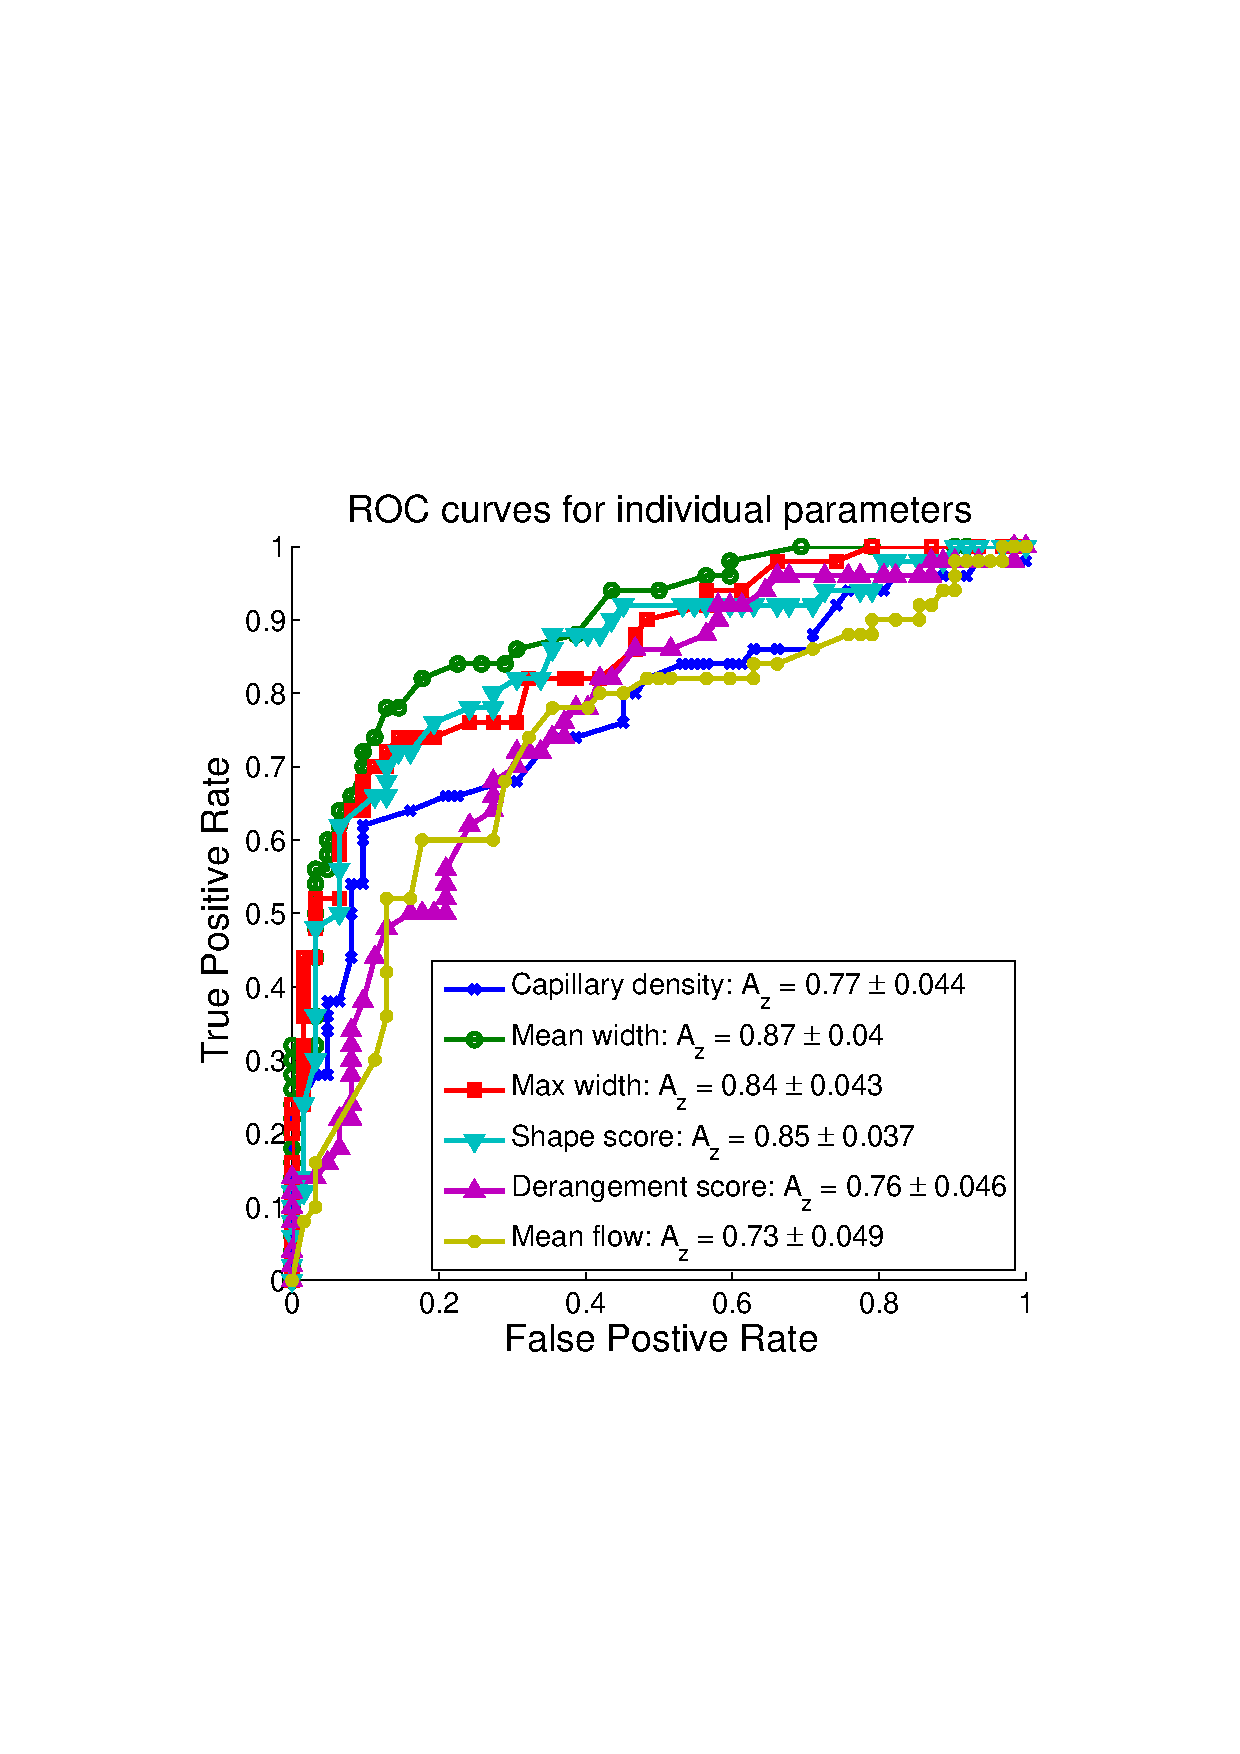
\includegraphics[width=0.48\columnwidth]{\figpath/individual_rocs.png} &
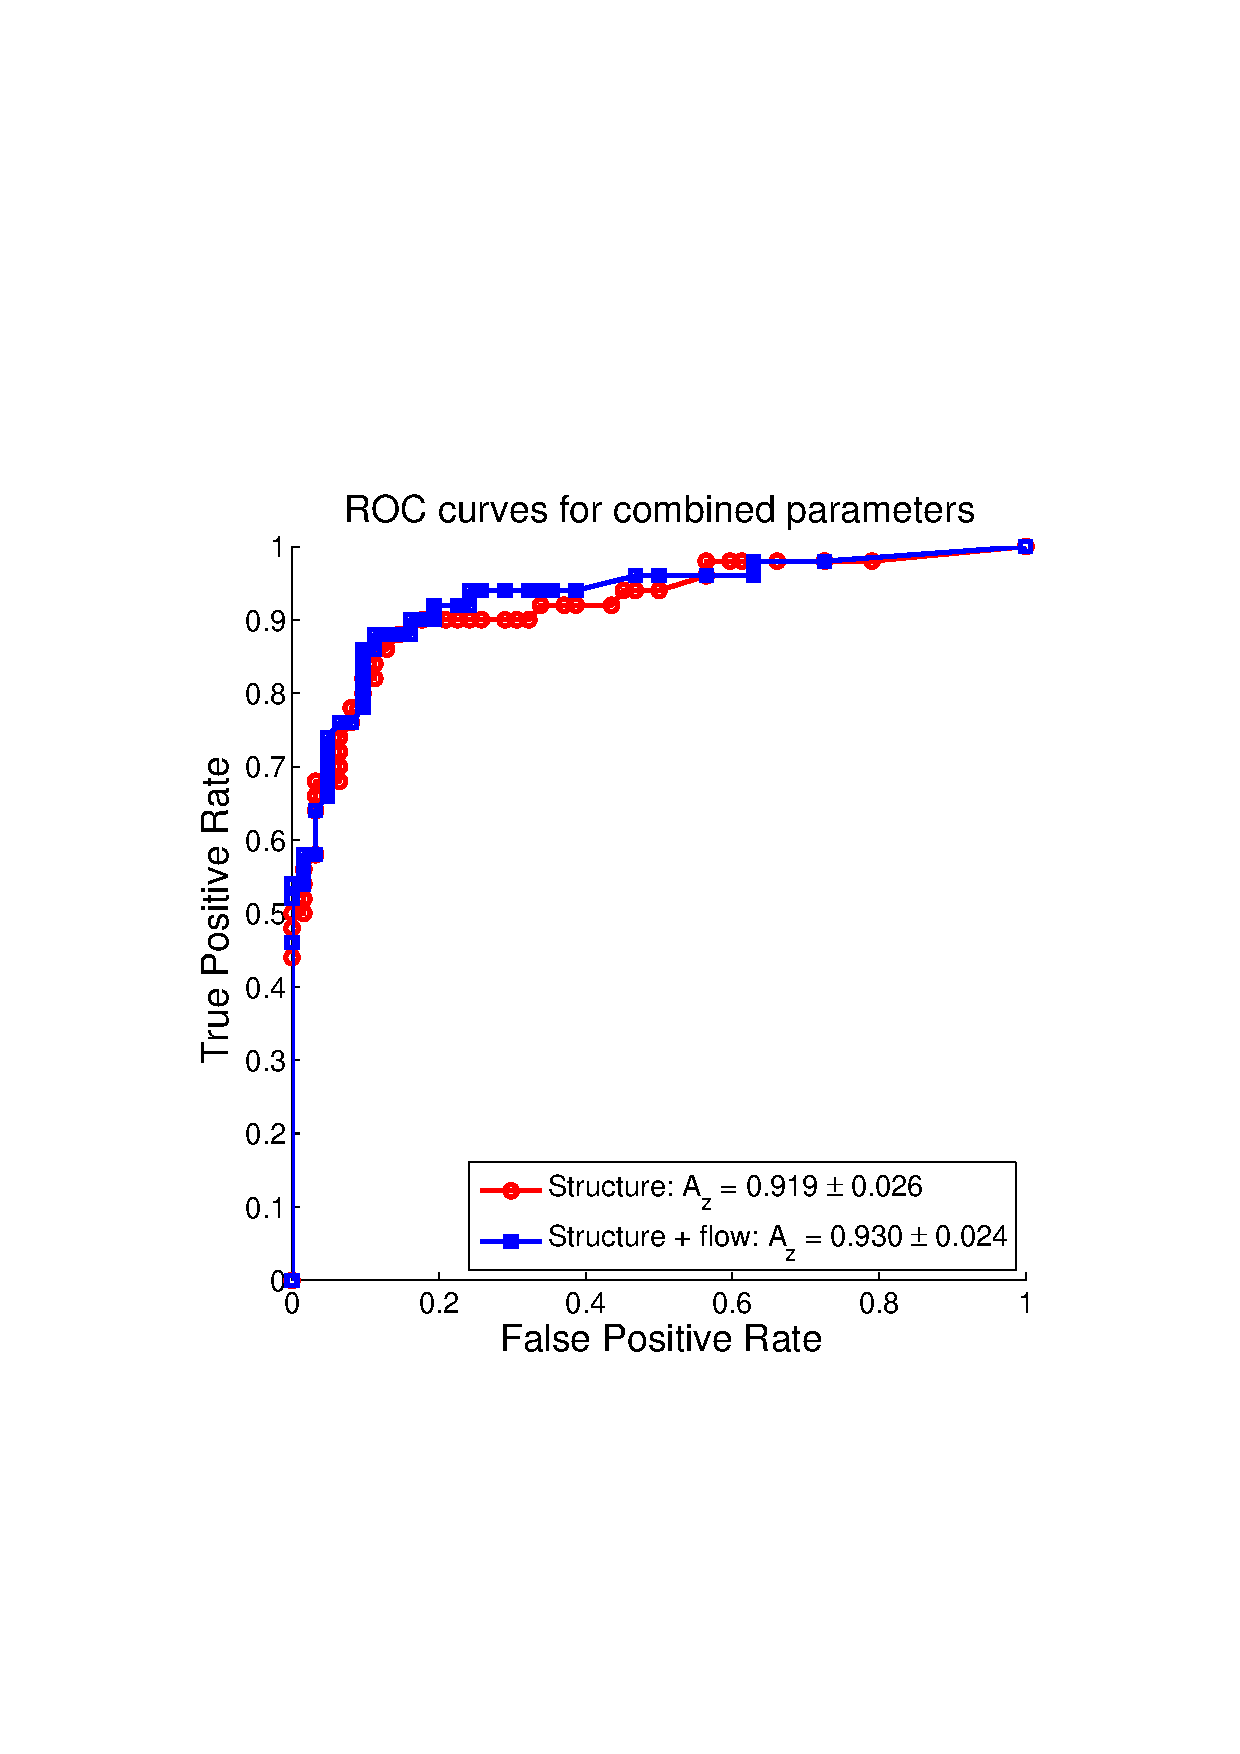
\includegraphics[width=0.48\columnwidth]{\figpath/combined_rocs.png} \\
(a) & (b)\\
\noalign{\smallskip}
\end{tabular}
%
\caption{ROCs for separating healthy controls and Primary Raynaud's from systemic sclerosis: %
(a) Indiviudal biomarkers; %
(b) Biomarkers combined in a logistic regression model.
}
\label{f:subject_rocs}
\end{figure}
%
Discussion of results.
%
\section{Conclusions}
\label{s:conclusions}
Conclusions.

%\textbf{Acknowledgements.}
%This work was funded by the Wellcome Trust. We are grateful to all the observers that annotated images used in the study.
%\end{document}

\bibliographystyle{splncs}
\bibliography{./bib/_aliases,./bib/miccai2016}

\end{document}
